\noindent\textbf{Difficulty:} Very hard (final)

\subsection{Level description}
The password is validated by an internal virtual machine. As the challenge itself says, you need to understand the bytecode rather than guess: identify the interpreter, its instruction set and the program that checks the password.

\begin{figure}[H]
\centering
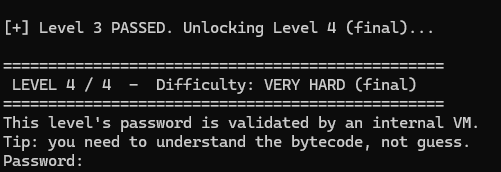
\includegraphics[width=0.7\linewidth]{initial/img/level4.png}
\caption{Level 3 passed and Level 4 (final) screen}
\label{fig:level4}
\end{figure}

\subsection{Static analysis}
% How the validation routine was located: strings, cross-references, relevant functions.
\textit{[To be completed.]}

\subsection{Dynamic analysis}
% Breakpoints used, registers/memory observed at the comparison.
\textit{[To be completed.]}

\subsection{Validation algorithm}
% Pseudocode of the rebuilt algorithm.
\textit{[To be completed.]}

\subsection{Solution (keygen)}
\textit{[To be completed.]}

\begin{lstlisting}[language=Python]
# Keygen - Level 4
# TODO: paste the keygen code
\end{lstlisting}

\subsection{Result}
Level under analysis. \textit{[To be completed.]}
